This project aims to improve performances of systems consisting of a layered data stack, able to handle large volumes of structured and unstructured data, at a high velocity, also defined as Big Data \cite{PDFBigData2024}. 
A generic data stack handles storing, management and retrieval of the data, offering access to those to the applications on top. However, there is no a single data stack for all cases, but different architectures used on different needs \cite{framptonCompleteGuideOpen2018,sakrBigDataProcessing2017,IcebergExamples2024}. The following Sections of this report defines the data stack for this use case, which is is illustrated in Figure \ref{fig:datastack}.

\begin{figure}[!ht]
    \begin{center}
      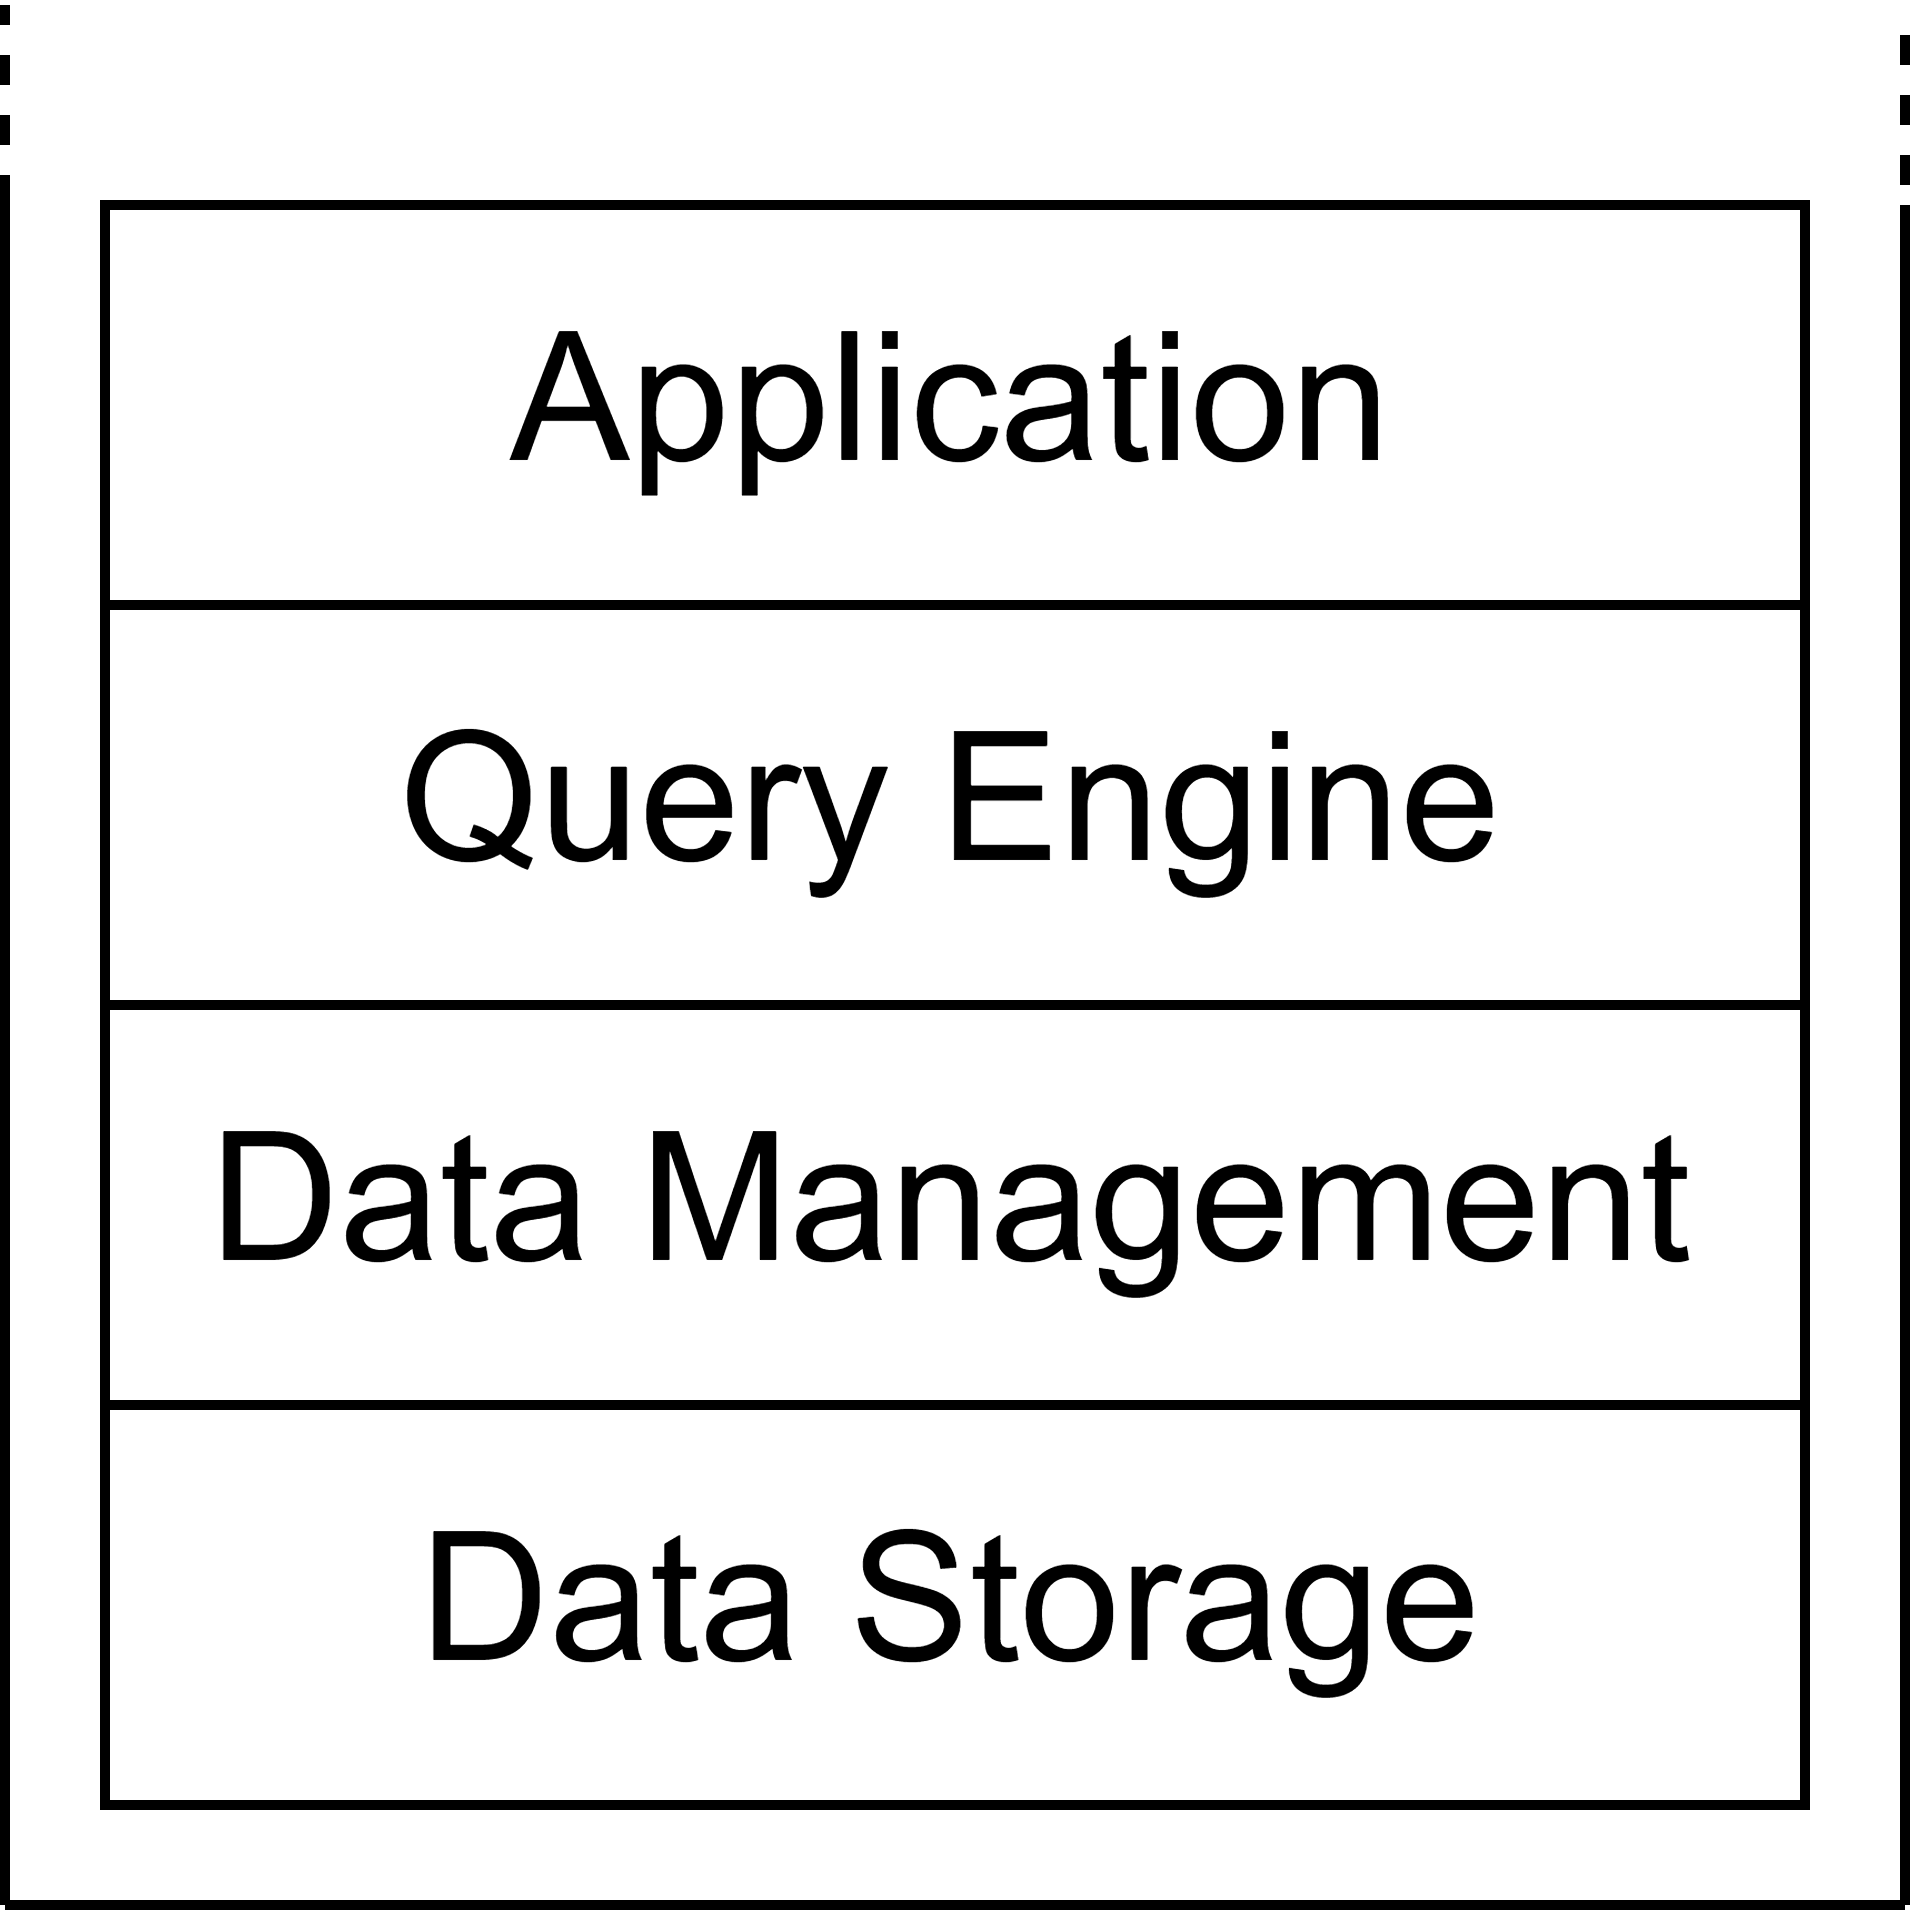
\includegraphics[width=0.4\textwidth]{figures/2-background_and_related_work/datastack.png}
    \end{center}
    \caption[Data stack abstraction]{Data stack abstraction for this project.}
    \label{fig:datastack}
\end{figure}

The data stack and this chapter are divided into four Sections:
\begin{enumerate}
    \item \textbf{Data Storage}: handles the physical storage of data. This layer determines how data is physically stored, including aspects like centralization or distribution, on-premise or cloud deployment, and storage formats such as files, objects, or blocks.
    \item \textbf{Data Management}: handles the organization, governance, and lifecycle of data. The data management layer may provide features such as \gls{ACID} properties, data versioning, support for open data formats, and the ability to store and manage both structured and unstructured data effectively.
    \item \textbf{Query Engine}: handles the execution of data queries. This layer is responsible for efficiently accessing, retrieving, and writing data based on user requests. Key features of a query engine may include caching mechanisms, highly scalable architectures, and support for diverse programming languages through \glspl{API}.
    \item \textbf{Application}: a system that utilizes the capabilities of the underlying data stack to achieve specific objectives. In this project, the focus will be on the Hopsworks feature store software.
\end{enumerate}

Following the data stack section, the architectures of the legacy system, IcedHops, and the delta-rs system architectures are explained in Section~\ref{sec:back_system_architecture}, showing how the technologies are reflected within the pipelines measured during this thesis' experiments.